\chapter{Práctica: Aparcamiento Automático}\label{cap.autoparking}
En este capítulo se describirá el desarrollo de una nueva práctica para la plataforma de JdeRobot, que se denominará ``Aparcamiento automático''. En este capítulo se aborda el desarrollo de la infraestructura, aplicación gráfica, así como el evaluador atomático que se ha creado y la solución realizada.  

\section{Enunciado}
El propósito de la práctica ``Aparcamiento automático'' es que un taxi autónomo sea capaz de aparcar en una plaza de aparcamiento sin chocar con los coches que están delante y detrás de la plaza libre de aparcamiento. El taxi dispondrá de un \acrshort{gps} que le proporciona una estimación de su posición en el entorno en que se encuentra. Este taxi constará de tres sensores láser mediante los cuales podrá obtener información acerca del entorno por el que se mueve. Este vehículo posee un actuador de movimiento que se basa en la velocidad de tracción y la velocidad de giro. Gracias a estos sensores y actuadores, el taxi podrá realizar un aparcamiento adecuado sin chocar con ningún vehículo.\\

En esta práctica el alumno deberá ser capaz de programar el comportamiento de este vehículo autónomo para que pueda aparcar. En la interfaz gráfica se puede visualizar un mapa del entorno por el que se mueve el taxi, así como la posición de este vehículo en el mapa. En esta interfaz, hay un visor que muestra gráficamente lo que ``ve'' cada láser del entorno. Esta interfaz facilitará al alumno la resolución de la práctica.\\

El algoritmo propuesto responde a un control reactivo, donde en cada momento el taxi actuará en función de los datos de los sensores o del algoritmo que se planifique en cada instante. El control reactivo permitirá controlar en todo momento el entorno que rodea al vehículo de forma que pueda responder ante situaciones imprevistas.

\section{Infraestructura}

En este apartado se describirá el entorno que se ha creado para poder realizar la práctica ``Aparcamiento automático''. Se comenzará describiendo el modelo de taxi empleado, así como los sensores y actuadores que posee el mismo. Después, se realizará una explicación del entorno por el cual se moverá el taxi.

\subsection{Taxi\_Holo\_Laser}
El robot que se ha empleado en esta práctica es un nuevo modelo basado en el modelo de taxi que se empleó en la práctica ``global\_navigation''. Este modelo de taxi se denomina taxi\_holo\_Laser. Es un robot que puede moverse de forma autónoma o teledirigida por un escenario. Este robot posee sensores \acrshort{gps} que le permiten saber cuál es su posición en todo momento; tiene tres sensores láser; así como motores que le permiten moverse por el escenario de manera adecuada.\\

Este modelo tiene las características propias de un automóvil, pero con el aspecto de un taxi. Las dimensiones de este taxi son de 4 metros de largo, 2 metros de ancho, y la altura es de 1.5 metros. El peso de este taxi es de 750 kg.  \\

Este taxi tiene tres sensores láser: uno se sitúa en la parte frontal del coche, otro en la parte trasera, y el último a la derecha del taxi. Este modelo de taxi lo podemos ver en la siguiente imagen.\\

\begin{figure}[H]
  \begin{center}
    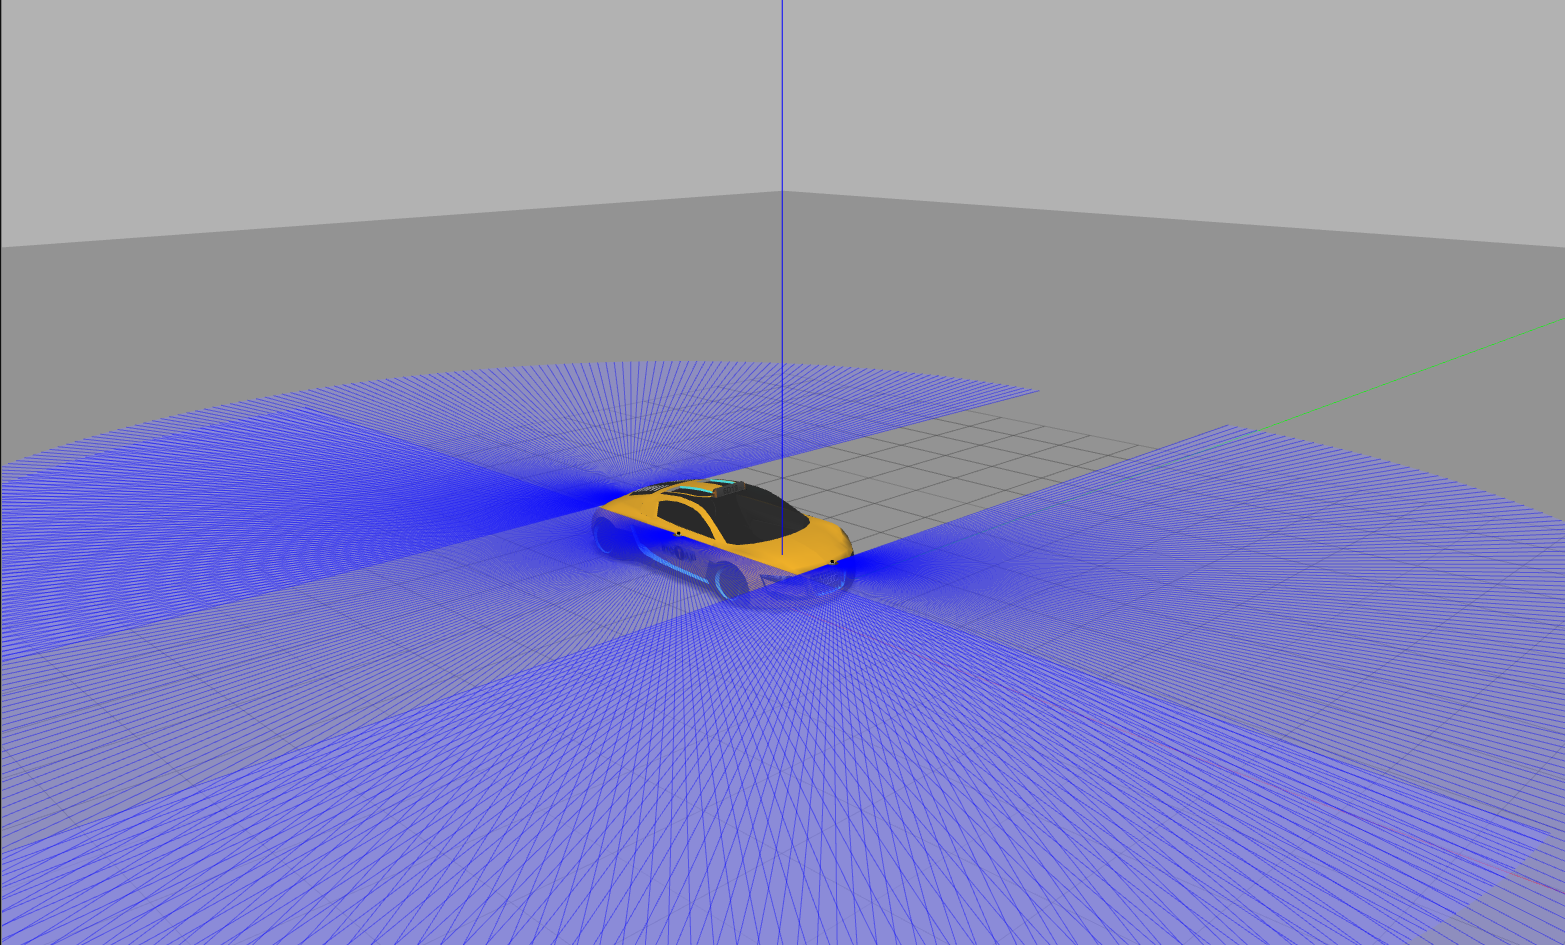
\includegraphics[width=0.6\textwidth]{figures/Autopark/taxiAutopark.png}
		\caption{Modelo taxi\_holo\_Laser}
		\label{fig.taxiAutopark}
		\end{center}
\end{figure}

\subsection{Sensores láser}
En este taxi se han instalado tres sensores láser como hemos mencionado antes. Un sensor se ha colocado en la parte frontal del vehículo, otro en la parte trasera, y el último en la parte derecha del taxi. Estos sensores serán empleados en el algoritmo de la práctica. Los sensores láser están formados por un array de 180 lasers, esto supone que vamos a tener un láser que puede medir distancia alrededor de 180 grados. Esta cualidad nos permite detectar obstáculos en estos 180 grados, y poder determinar dónde se encuentra aproximadamente. Las medidas de distancia que nos devuelve el láser están en milímetros. \\

Como sucede en las anteriores prácticas, la plataforma JdeRobot encapsula la complejidad de los sensores y nos devuelve los datos que ofrecen (los datos de distancia).\\

En esta práctica se han empleado los drivers:

\begin{itemize}
\item holoCarPose3D: Los componentes emplean este plugin para obtener su posición en tiempo real. Este plugin también se utiliza para cambiar la posición de los componentes.
\item	holoCarMotors: El componente interactúa con este plugin. Este plugin permite dotar al componente de velocidad, tanto velocidad de tracción como velocidad de rotación y modifica los datos de la interfaz de usuario.
\item	laser: Este plugin será empleado por los componentes para obtener datos de la distancia que hay hasta los obstáculos.
\end{itemize}

\subsection{Modelo acera} \label{sec.acera}
El objetivo de la práctica es que el taxi sea capaz de aparcar de forma autónoma. Para ello es necesario crear un entorno donde se moverá el taxi. Esto supone que se deben crear los modelos necesarios para poder crear el entorno. El taxi deberá aparcar paralelo a una acera, por lo tanto, se ha creado el modelo ``acera''. Este modelo se puede ver en la siguiente imagen.

\begin{figure}[H]
  \begin{center}
    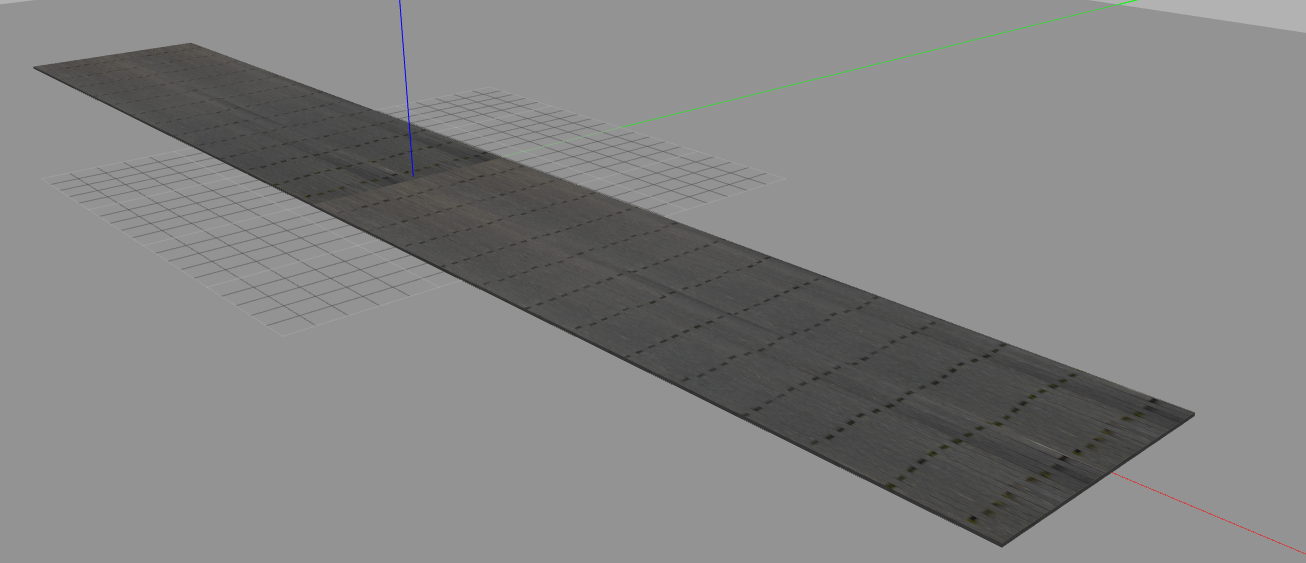
\includegraphics[width=0.7\textwidth]{figures/Autopark/acera.png}
		\caption{Modelo acera}
		\label{fig.acera}
		\end{center}
\end{figure}

\subsection{Modelo carNoMotor}
Como hemos mencionado en el Apartado~\ref{sec.acera}, es necesario crear los modelos que se van a emplear para poder crear el entorno (mundo de Gazebo) donde se moverá el taxi. El taxi deberá aparcar entre dos coches, y habrá más coches estacionados. Por este motivo se ha creado el modelo ``carNoMotor'', el cual como su propio nombre indica no posee motores, ya que queremos que esté estacionado. Este modelo se utilizará varias veces al crear el mundo de Gazebo. A continuación, podemos ver en una imagen este modelo.

\begin{figure}[H]
  \begin{center}
    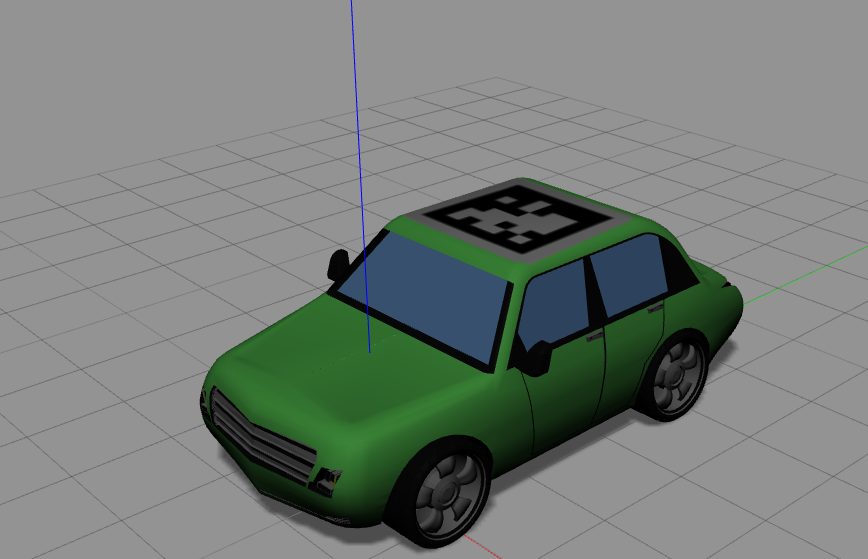
\includegraphics[width=0.5\textwidth]{figures/Autopark/carNoMotor.png}
		\caption{Modelo carNoMotor}
		\label{fig.carNoMotor}
		\end{center}
\end{figure}

\subsection{Mundo de Gazebo}
La creación de un mundo de Gazebo es necesaria para poder ver cómo aparca el taxi en el entorno. Este mundo estará formado por un modelo de carretera (road) que tiene Gazebo, poseerá dos aceras para lo cual emplearemos el modelo ``acera'', además se emplearán varios coches del modelo ``carNoMotor'' que estarán aparcados; y, por último, se incluirá el modelo del taxi (taxi\_holo\_Laser), que realizará la solución que le indiquemos. Para poder tener este escenario se ha creado un mundo en Gazebo llamado ``autopark.world''. Este archivo tiene el siguiente aspecto:

\vspace{20pt}
	\begin{lstlisting}[frame=single]
<?xml version="1.0"?>
<sdf version="1.4">
  <world name="default">

    <scene>
      <grid>true</grid>
    </scene>

    <!-- A global light source -->
    <include>
      <uri>model://sun</uri>
    </include>

    <!-- Ground -->
    <include>
      <uri>model://ground_plane_sincolor</uri>
    </include>
    <include>
      <uri>model://acera</uri>
      <pose>5 9 0 0 0 0</pose>
    </include>
    <include>
      <uri>model://acera</uri>
      <pose>5 -9 0 0 0 0</pose>
    </include>

    <!-- A taxi with lasers-->
    <include>
      <uri>model://taxi_holo_Laser</uri>
      <pose>-7 2.5 0 0 0 0</pose>
    </include>

    <!-- Cars -->
    <include>
      <uri>model://carNoMotor</uri>
      <pose>-20 -3 0 0 0 1.57</pose>
    </include>
    <include>
      <uri>model://carNoMotor</uri>
      <pose>-13.5 -3 0 0 0 1.57</pose>
    </include>
    <include>
      <uri>model://carNoMotor</uri>
      <pose>-7 -3 0 0 0 1.57</pose>
    </include>
    <include>
      <uri>model://carNoMotor</uri>
      <pose>0.5 -3 0 0 0 1.57<pose>
    </include>
    <include>
      <uri>model://carNoMotor</uri>
      <pose>14 -3 0 0 0 1.57</pose>
    </include>
    <include>
      <uri>model://carNoMotor</uri>
      <pose>21.5 -3 0 0 0 1.57</pose>
    </include>
    <include>
      <uri>model://carNoMotor</uri>
      <pose>29 -3 0 0 0 1.57</pose>
    </include>

    <!-- A Road -->
    <road name="my_road_1">
      <width>10</width>
      <point>-25 0 0.02</point>
      <point>35 0 0.02</point>
    </road>

  </world>
</sdf>
	\end{lstlisting}


En la siguiente imagen podemos ver cuál es el aspecto que tiene el mundo que hemos creado en Gazebo.

\begin{figure}[H]
  \begin{center}
    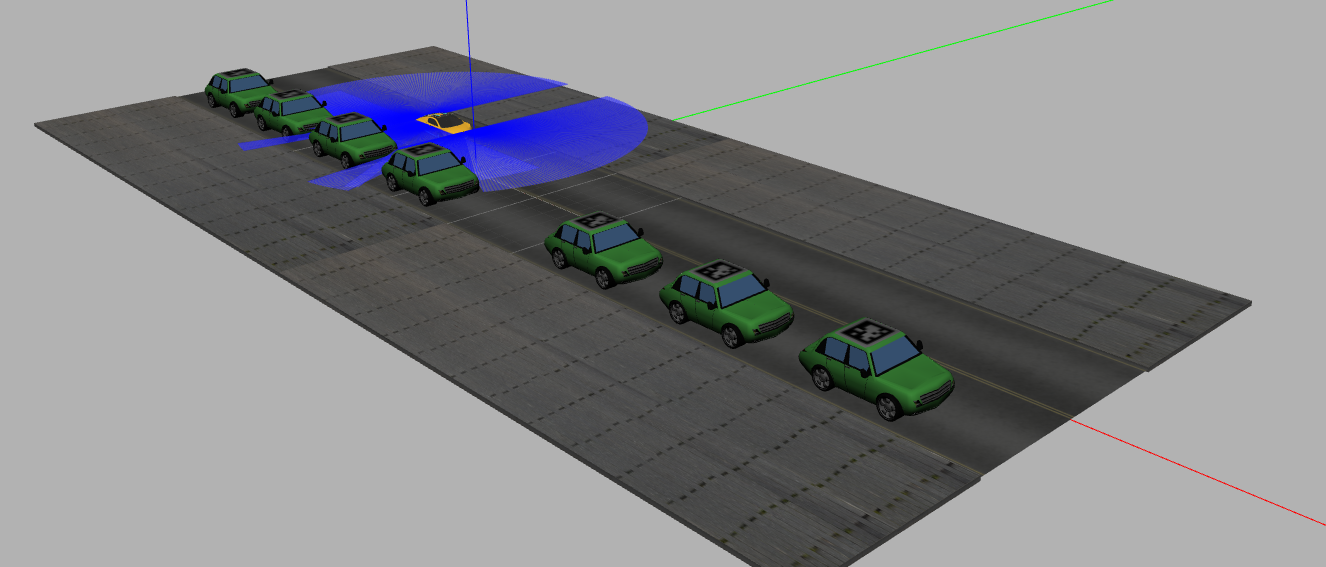
\includegraphics[width=0.8\textwidth]{figures/Autopark/Mundo_Autopark.png}
		\caption{Mundo autopark.world en Gazebo}
		\label{fig.Mundo_Autopark}
		\end{center}
\end{figure}

\section{Componente Académico}
El componente académico resuelve diversas funcionalidades en la práctica: ofrece una interfaz gráfica al usuario, que le ayuda a depurar su código; ofrece acceso a sensores y actuadores en forma de métodos simples (oculta el middleware de comunicaciones); incluye código auxiliar que no es el centro del algoritmo y que ayuda a programar la solución. El componente deja todo listo para que el estudiante sólo tenga que retocar en MyAlgorithm.py.\\

Este componente ofrece al programador del algoritmo un \acrshort{api} de sensores y actuadores. A continuación, se puede ver el \acrshort{api} específico de esta práctica:

\begin{itemize}
\item pose3d.getX(): Permite obtener la posición del robot en el eje X.
\item	pose3d.getY(): Permite obtener la posición del robot en el eje Y.
\item	pose3d.getYaw(): Permite obtener la orientación del robot con respecto al mapa.
\item	laser.getLaserData(): Permite obtener los datos del sensor láser, que se compone de 180 pares de valores (0-180º, distancia en milímetros).
\item motors.sendV(): Para establecer la velocidad lineal.
\item	motors.sendW(): Para establecer la velocidad de giro.
\end{itemize}

Es necesario crear un archivo de configuración en la práctica. Este archivo sirve para poder indicar los puertos que utilizan cada uno de los plugins que posee el taxi que vamos a emplear. Este archivo es necesario para que nuestra aplicación pueda comunicarse con gazeboserver. El archivo de configuración (autopark.cfg) en la práctica tiene el siguiente aspecto:

\vspace{20pt}
	\begin{lstlisting}[frame=single]
Autopark.Motors.Proxy  = Motors:default -h localhost -p 9999
Autopark.Pose3D.Proxy  = Pose3D:default -h localhost -p 9989
Autopark.Laser1.Proxy  = Laser:default -h localhost -p 8996
Autopark.Laser2.Proxy  = Laser:default -h localhost -p 8997
Autopark.Laser3.Proxy  = Laser:default -h localhost -p 8998

Autopark.Motors.maxV = 250
Autopark.Motors.maxW = 20

	\end{lstlisting}


En el caso del taxi podemos ver que los motores emplean el puerto 9999, el Pose3D emplea el puerto 9989, y los sensores láser utilizan los puertos 8996, 8997, 8998. En este archivo se indica también la velocidad lineal máxima y la velocidad angular máxima.\\

En la práctica el comportamiento se divide en varias tareas. Para poder realizar estas tareas simultáneamente, empleamos hilos de ejecución. En concreto, esta práctica emplea tres procesos diferentes:

\begin{itemize}
\item Hilo de control: Este hilo se encarga de actualizar los datos de los sensores y los actuadores a través de las interfaces \acrshort{ice}. El tiempo de actualización de este hilo es un punto muy importante que hay que tener en cuenta, ya que este componente establece la velocidad y la dirección del robot en todo momento. Este intervalo de actualización debe ser un periodo de tiempo muy corto. Si este tiempo fuera muy grande, las decisiones que modifican la trayectoria del robot podrían influir en su comportamiento, haciendo que la trayectoria sea incorrecta. En esta práctica el hilo de control de actuadores y sensores se actualizará cada vez que se actualice la \acrshort{gui}, es decir, cada 50 ms.
\item	Hilo de la interfaz gráfica de usuario (\acrshort{gui}): Se encarga de actualizar la interfaz gráfica. Este hilo consta de los manejadores de eventos del \acrshort{gui}, que son los encargados de ejecutar el código del fichero MyAlgorithm.py. El intervalo de actualización de la interfaz gráfica debe ser corto, puesto que se tiene que mostrar la posición del robot en el mapa que muestra la interfaz en tiempo real. El intervalo de actualización es de 50 ms.

\end{itemize}

\subsection{Interfaz gráfica de la práctica}
La interfaz gráfica de usuario (\acrshort{gui}) se emplea, en la práctica, para representar información que pueda ayudar a resolver el algoritmo planteado. Esta interfaz sirve para poder ejecutar el código que da solución a la práctica. Esta interfaz, como se mencionó en las prácticas anteriores, es programada en PyQt5.\\

Esta \acrshort{gui} contiene un lienzo en blanco (como si fuera una imagen) donde se ha pintado parte del mundo de Gazebo, así como la posición del coche. En concreto, en este lienzo se puede ver que hay ciertas partes pintadas en negro, que se corresponden con las aceras y los coches aparcados, es decir, los obstáculos. Por el contrario, las zonas que aparecen en blanco es donde no hay obstáculos, es decir, la carretera sin objetos. El taxi aparece representado mediante un rectángulo amarillo con ruedas en negro. Este rectángulo también rota cuando el taxi lo hace, de esta forma se puede representar adecuadamente el comportamiento del taxi. En este pequeño mapa del escenario podemos ver que aparecen pintadas de verde las aristas de un rectángulo, el cual se corresponde con la posición ideal que debería conseguir el taxi al aparcar. En este mapa también podemos observar unos puntos rojos que aparecen consecutivamente, los cuales se corresponden con la estela del taxi, es decir, se corresponden con las posiciones que ha tenido el taxi. Pero todas las posiciones que tiene el taxi no se pintan, solamente se pintan las últimas. Esto se debe a que hemos creado un array de cierto tamaño para poder representar únicamente unos cuantos puntos y no todos. Este array es un ``array circular'', es decir, es una array en el cual vamos añadiendo las nuevas posiciones por el final del array y cuando llega a un cierto tamaño vamos borrando la primera posición del array y desplazando el contenido de sus posiciones a una posición anterior. De esta forma podemos insertar nuevos puntos por el final e ir borrando las posiciones anteriores por las que ha pasado el taxi.\\

A la derecha de este mapa, se representa el taxi mediante un rectángulo amarillo (con sus ruedas en negro), y se muestran los datos que ofrecen los sensores láser. Cada sensor láser se ha pintado de un color diferente para distinguirlos. Si comparamos esta representación con el mundo de Gazebo se podría ver que la representación es idéntica a cómo se ven los sensores láser en Gazebo. Para poder representar cada uno de los sensores láser en la posición adecuada se han empleado matrices de rotación y traslación al igual que sucedía en otras prácticas. Se puede ver en la imagen que hay al final de este punto~\ref{fig.GUI_Autopark} cómo se representan perfectamente los sensores y el coche empleando este tipo de matrices. \\

A la derecha de la representación del taxi con los sensores láser, tenemos un teleoperador para poder teleoperar el robot. Este teleoperador controla las velocidades lineal y angular del robot. La velocidad lineal del robot se puede controlar moviendo el joystick en sentido vertical. Cuanto más subamos el joystick más velocidad tendrá el robot hacia delante, y si lo bajamos del todo más velocidad lineal tendrá el robot hacia atrás. La velocidad angular del robot se controla moviendo el joystick en sentido horizontal, según lo movamos a izquierda o a la derecha, el robot girará en un sentido u otro.\\

En la esquina superior derecha de la \acrshort{gui}, aparece representada una imagen del logo de JdeRobot. Esta imagen es RGB y ha sido escalada.\\

En la interfaz aparecen dos botones que son muy importantes para la práctica. El botón de debajo del mapa que muestra una parte del entorno, es el botón que nos permitirá ejecutar el código de solución a la práctica. Este botón, también nos permitirá parar el código de la solución, de forma que el taxi se quede parado donde estuviera situado.\\

El botón que aparece debajo de la gráfica con los sensores láser y el teleoperador, es el botón que nos permitirá parar el robot si lo estamos teledirigiendo con el teleoperador. Este botón le ordenará al vehículo que mantenga velocidad de tracción y rotación nula.\\

A continuación, podemos ver una imagen de la interfaz gráfica, donde se muestran todos estos elementos que acabamos de describir.

\begin{figure}[H]
  \begin{center}
    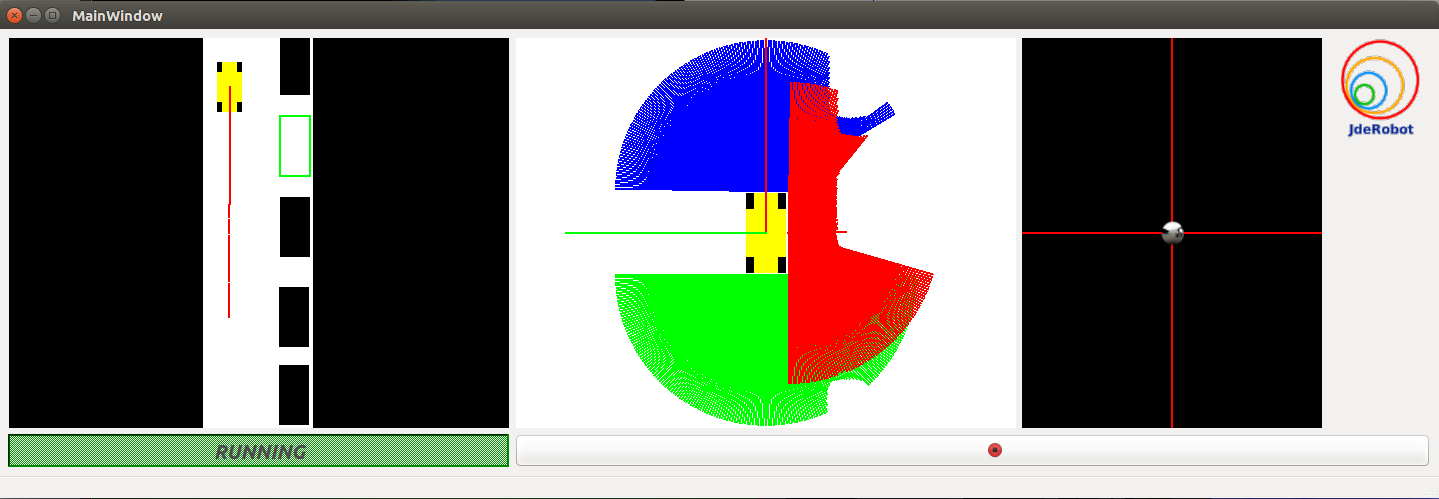
\includegraphics[width=0.9\textwidth]{figures/Autopark/GUI_Autopark.png}
		\caption{\acrshort{gui} del Autopark}
		\label{fig.GUI_Autopark}
		\end{center}
\end{figure}

\section{Solución de referencia}
En esta sección se describirá cómo aparcan los coches autónomos reales, así como la solución ``ad hoc'' que se ha realizado para la práctica. Tras esto, se explicarán algunos experimentos realizados. 

\subsection{Cómo aparcan los coches autónomos reales}
Durante la conducción, una de las maniobras más complicadas es el aparcamiento del vehículo, en especial en ciertas zonas donde los huecos disponibles son bastantes escasos. En la actualidad existen distintos avances tecnológicos para facilitar el aparcamiento al conductor.\\


El primer prototipo de coche con aparcamiento autónomo fue producido en Francia, hace alrededor de 20 años por el INRIA (Institut National de Recherche en Informatique et en Automatique). Este prototipo fue el primero en realizar un aparcamiento autónomo en paralelo. Hoy en día, cada vez más fabricantes de vehículos incorporan esta tecnología, pero todos se basan en los avances de INRIA, el cual estableció un estándar. El código de este estándar es J3016, que establece cinco niveles de aparcamiento autónomo según la capacidad del vehículo. Además, existe el nivel 0, que no tiene capacidad autónoma.

\begin{itemize}
\item Nivel 0: No hay automatización de la conducción. Las tareas de conducción son realizadas en su totalidad por el conductor.
\item	Nivel 1: Asistencia al conductor. El vehículo tiene algún sistema de automatización de la conducción, ya sea para el control de movimiento longitudinal o el movimiento lateral, pero no ambas cosas al mismo tiempo. El conductor realiza el resto de tareas de conducción. El sistema no cuenta con detección y respuesta ante objetos y eventualidades de forma completa. Esta tarea recae sobre el conductor, por lo que el conductor debe estar siempre atento.
\item	Nivel 2: Automatización parcial. El vehículo posee sistemas de automatización de la conducción para el control de movimiento longitudinal y el movimiento lateral, ambas cosas al mismo tiempo. El sistema no cuenta con detección y respuesta ante objetos y eventualidades de forma completa. Esta tarea recae sobre el conductor, por lo que el conductor debe estar siempre atento como en el nivel 1.
\item	Nivel 3: Automatización condicional. En este nivel el vehículo presenta sistemas de automatización para el control de movimiento lateral y longitudinal. El sistema tiene detección ante objetos y eventos y puede responder ante ellos. En este nivel el usuario deberá estar preparado para intervenir si el sistema lo solicita o se produce un fallo o pérdida de las condiciones de funcionamiento. Si se produce alguna de estas situaciones, el usuario se convierte en conductor.
\item Nivel 4: Alta autonomía. En este nivel el sistema cuenta tanto con los sistemas de automatización presentes en el anterior nivel, como con sistemas de detección de objetos y eventos. Además, es capaz de responder ante ellos. El sistema de automatización de la conducción tiene un sistema de respaldo para actuar en caso de fallo del sistema principal y poder conducir hasta una situación de riesgo mínimo. En algunas situaciones es posible que el vehículo no siga conduciendo.
\item	Nivel 5: Autonomía total. Este nivel cuenta con todos los beneficios del sistema de automatización del nivel 4. Sin embargo, la diferencia es que en este caso el vehículo podría seguir conduciendo en todo momento o circunstancia.

\end{itemize}

La tecnología que se emplea para el aparcamiento autónomo tiene que tener en cuenta diversos factores para poder aparcar: espacio disponible, maniobras a realizar y posición. Para conseguir este objetivo los coches emplean sensores que llevan incorporados. Un sistema de aparcamiento automático requiere de sensores que midan la distancia desde el coche hasta los límites de la plaza y los otros coches u obstáculos, tanto en el parachoques trasero como en el parachoques delantero.\\

Estos sensores suelen ser de ultrasonidos, y su número y distribución depende del tamaño y diseño del coche, aunque suelen ser cuatro o cinco por parachoques. En algunas ocasiones se puede emplear un radar como sensor.\\

En los laterales de los paragolpes es necesario que haya más sensores orientados de forma transversal. De esta forma pueden medir la distancia hacia el lateral del coche. Estos sensores permiten identificar si existe un hueco en el que aparcar y permiten al sistema identificar si el tamaño del hueco es suficiente para que el coche entre.\\

La firma Bosch lidera el suministro de tecnología para la automoción y tiene a la totalidad de marcas fabricantes de automóviles como clientes. Un sistema que Bosch proporciona a las marcas es la ``cámara de marcha atrás''. Esta cámara está ubicada en la parte posterior del vehículo, y se activa de forma automática cuando el conductor da marcha atrás. Inmediatamente aparecen imágenes en color del entorno en el monitor y las líneas límite de maniobra para evitar roces, así como advertencias acústicas.\\

Otro sistema importante de Bosch es el sistema Multi-cámara, que cuenta con cuatro cámaras con apertura de 190º que captan todo el entorno del vehículo y se reflejan en la pantalla del salpicadero. Estas imágenes son imágenes en 3D sin distorsión.\\

Bosch también incorpora un dispositivo llamado ``freno de emergencia en maniobras''. Este dispositivo detecta obstáculos y objetos en movimiento (mediante sensores ultrasonidos) hasta una distancia de cuatro metros y a una velocidad de no más de 10 km/h. Si hay riesgo de colisión avisa al conductor y si este no reacciona, activa una frenada de emergencia.\\

Estas son algunas de las tecnologías que emplean los coches autónomos o parcialmente autónomos en aparcamiento. Con estos sensores los vehículos son capaces de realizar maniobras complicadas, que a las personas nos resultan más tediosas. Las tecnologías avanzan rápido, y en este campo han avanzado mucho desde el inicio. Ya existen coches como el coche de Google que son autónomos por completo, aunque no se hayan comercializado aún por motivos de leyes. Quizás en algún futuro iremos en el coche tranquilamente como pasajeros y este vehículo nos llevará al destino de forma adecuada.

\subsection{Solución desarrollada}
En esta práctica hemos desarrollado una solución ``ad hoc'' que resuelve el problema del aparcamiento autónomo. Esta solución se basa en los datos que ofrecen los sensores láser para saber cuál es la situación del taxi en el entorno y tomar las decisiones que tienen que ver con el aparcamiento. La solución que se ha implementado se describe a continuación.\\

La solución se programa en el fichero MyAlgorithm.py, en el método ``execute'', que se ejecuta periódicamente. Esto permite que la práctica se ejecute como un control reactivo, donde el taxi recoge los datos de los sensores en cada instante y toma decisiones basándose en estos datos. En esta práctica no se realiza ningún tipo de planificación (como sucedía en la práctica ``TeleTaxi'') antes del pilotaje, sino que se realiza el pilotaje directamente.\\


En la solución que se ha desarrollado el taxi obtendrá los datos que le proporciona cada láser en primer lugar. Para obtener estos datos, se emplea la función laser.getLaserData() para cada correspondiente láser. Esta función nos devuelve los datos del sensor láser, los cuales consisten en 180 pares de valores (distancia y ángulo). El siguiente paso ha sido hacer una media de los 180 valores del láser para tener conocimiento de cuál es la situación del coche. \\

Al comienzo de la ejecución de la práctica el taxi se encontrará estacionado más atrás de la plaza de aparcamiento, como se puede ver en la siguiente imagen.

\begin{figure}[H]
  \begin{center}
    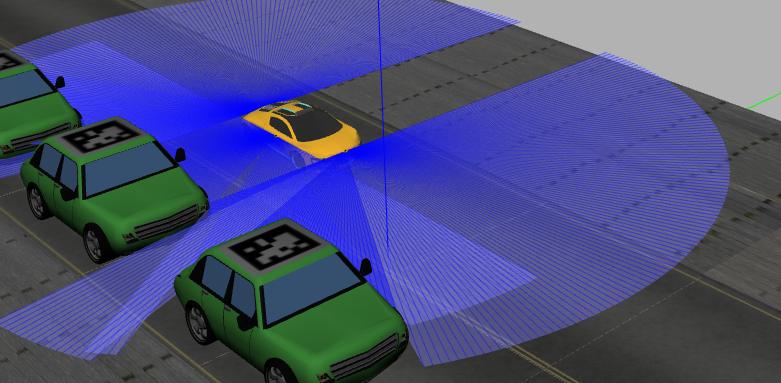
\includegraphics[width=0.7\textwidth]{figures/Autopark/Posicion1.png}
		\caption{Posición inicial del taxi en la práctica}
		\label{fig.Posicion1}
		\end{center}
\end{figure}

Los datos del láser son comprobados en cada iteración, ya que son los que proporcionan al taxi la información del entorno. El coche emplea velocidad constante si no ha encontrado aún ninguna plaza de aparcamiento libre. El taxi comprobará la distancia del láser de la derecha y el láser del parachoques trasero para ver si puede parar y estacionar el vehículo. Si los dos láseres tienen un valor entre un rango de valores significa que el taxi ha encontrado una plaza de aparcamiento libre. El taxi parará en paralelo al coche de delante de la plaza de aparcamiento un momento antes de comenzar a aparcar. Podemos ver en la siguiente imagen cómo el taxi alcanza el vehículo de delante de la plaza y para.

\begin{figure}[H]
  \begin{center}
    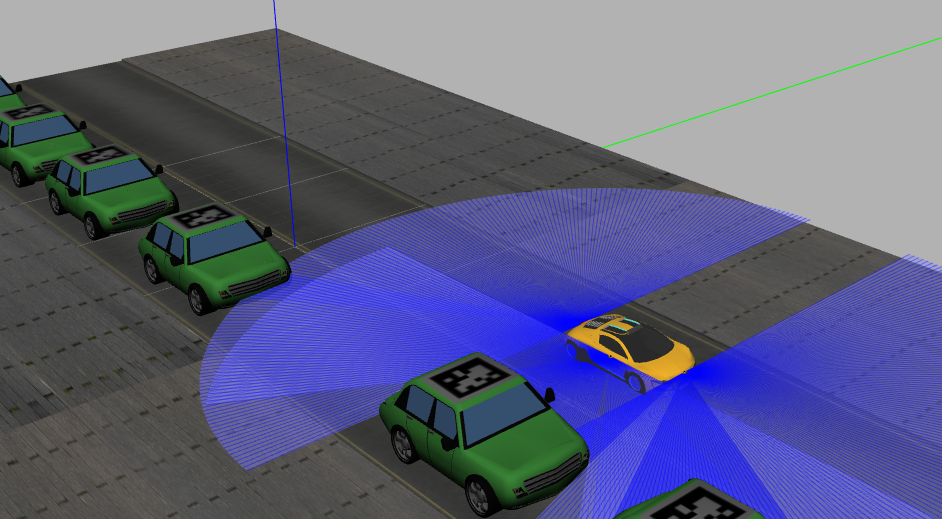
\includegraphics[width=0.7\textwidth]{figures/Autopark/Posicion2.png}
		\caption{Posición al parar en paralelo al coche de delante de la plaza libre}
		\label{fig.Posicion2}
		\end{center}
\end{figure}

Cuando el taxi ya está parado en paralelo al coche de delante de la plaza de aparcamiento, entonces comienza la maniobra de aparcamiento. Al principio el taxi comenzará a dar marcha atrás lentamente, es decir, con una velocidad de tracción determinada. Pero también tendrá cierta velocidad de giro, con lo que el coche describirá una especie de arco al aparcar (como lo hace un coche real al comenzar a aparcar en paralelo). El giro será hacia la derecha hasta que tiene una determinada inclinación. Esta maniobra la podemos ver en la imagen siguiente.

\begin{figure}[H]
  \begin{center}
    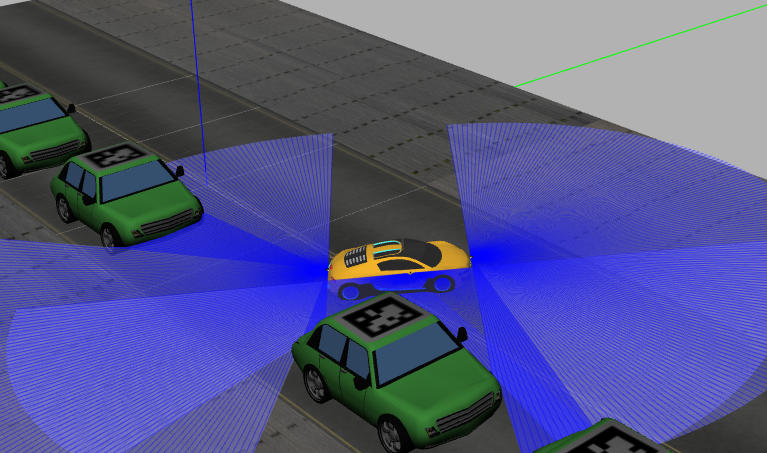
\includegraphics[width=0.7\textwidth]{figures/Autopark/Posicion3.png}
		\caption{Posición al dar marcha atrás con giro a la derecha}
		\label{fig.Posicion3}
		\end{center}
\end{figure}

Cuando el coche alcanza una determinada orientación, entonces es hora de realizar otra maniobra para poder enderezar el vehículo. Ahora que ya ha entrado parte del coche en la plaza de aparcamiento, el taxi dará marcha atrás y realizará otra especie de arco. Es decir, que en esta ocasión el coche tendrá una velocidad de giro, pero girando hacia la izquierda. Esta maniobra se puede ver en la imagen siguiente.

\begin{figure}[H]
  \begin{center}
    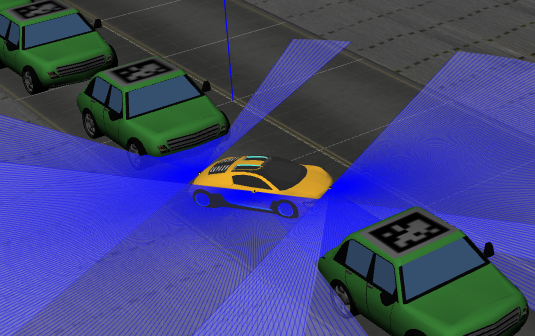
\includegraphics[width=0.7\textwidth]{figures/Autopark/Posicion4.png}
		\caption{Posición al dar marcha atrás con giro a la izquierda}
		\label{fig.Posicion4}
		\end{center}
\end{figure}

El taxi comprobará los datos del láser trasero en todo momento para saber si está cerca del coche de atrás. El coche seguirá marcha atrás y girando hacia a la izquierda hasta que detecte que está demasiado cerca del coche de atrás. Cuando detecte esta situación, entonces parará y comenzará a rectificar. Para poder realizar la rectificación dará marcha hacia delante muy despacio y girando hacia la derecha. Esta maniobra la realiza hasta quedar recto, es decir, de forma paralela a la acera. Cuando esté paralelo a la acera, el taxi comprobará con los sensores láser frontal y trasero si se ha quedado muy pegado a un coche u otro. Si el taxi se ha quedado muy cerca del coche de atrás y tiene mucho margen por delante, entonces dará marcha hacia delante hasta quedar más o menos centrado en la plaza de aparcamiento. En caso contrario, el taxi estaría muy pegado al coche de delante, y daría marcha atrás hasta estar centrado. Cuando el coche detecte que se ha quedado centrado en la plaza de aparcamiento, entonces parará. A continuación, se puede observar como ha quedado el taxi perfectamente estacionado.

\begin{figure}[H]
  \begin{center}
    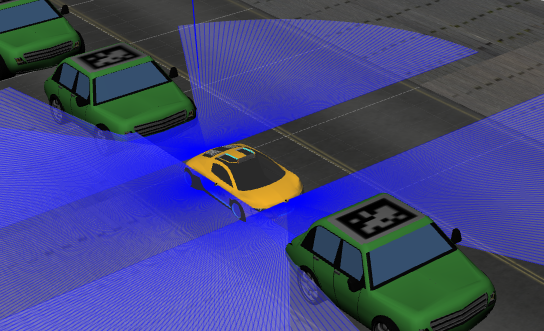
\includegraphics[width=0.7\textwidth]{figures/Autopark/Posicion5.png}
		\caption{Taxi estacionado}
		\label{fig.Posicion5}
		\end{center}
\end{figure}


\section{Evaluador automático}
La práctica tiene un evaluador automático, que permite calificar la solución a la práctica teniendo en cuenta diferentes parámetros. El evaluador automático muestra estos parámetros en una interfaz gráfica, así como la nota que obtiene el alumno. Al igual que la aplicación gráfica, el evaluador automático se ha creado empleando PyQt5. Como sucedía en las anteriores prácticas, el evaluador automático se ha creado mediante clases, que serán instanciadas en una clase principal. A continuación, se describe cómo es el evaluador automático.\\

En la esquina superior izquierda de la interfaz, hay un visor que muestra un reloj digital. Este reloj va mostrando los segundos que han pasado desde que se ha ejecutado la práctica. Es decir, los segundos se inicializan a 0 y van aumentando según pasa el tiempo.\\

En la esquina inferior izquierda de la interfaz gráfica, se representa parte de un círculo formado por diferentes colores, donde hay una aguja que apunta a cierto sitio dependiendo de la ocasión. Este semicírculo representa la orientación del robot, en función de determinados colores. Esto nos permite ver si nuestro vehículo está correctamente alineado o si por el contrario está algo desviado. Para que el coche esté perfectamente alineado tiene que tener una orientación de 0 grados. Pero para poder pintar el semicírculo se ha decidido poner la orientación correspondiente a 0 grados en la parte superior, por lo que a la orientación debemos sumarle pi/2 para poder representarla adecuadamente. El color verde representa una orientación entre -15 y 15 grados. La zona anaranjada representa dos rangos de valores para la orientación. Por un lado, representa el rango de orientación entre -45 y -15 grados; y, por otro lado, representa el rango de orientación entre 15 y 45 grados. El color rojo representa una orientación entre -45 y 45 grados. La aguja apuntará a un color u otro, y a cierta zona en función de la orientación que posea el robot.\\

En la esquina superior derecha, se muestra en el visor diferentes distancias. Las distancias que se muestran son: la distancia a la acera que está pegada a la zona de aparcamiento, la distancia al coche de delante del hueco de aparcamiento, y la distancia al coche de atrás del hueco de aparcamiento. Esto nos permite comprobar la distancia que tenemos a los coches de delante y detrás y podemos ver si nos estamos acercando mucho a alguno de estos coches al realizar el aparcamiento, lo que podría ser peligroso, ya que podríamos colisionar con alguno de ellos.\\

Debajo de los mensajes de distancias, el visor tiene una barra de progreso. Esta barra (de color rojo) aumentará en caso de que nos choquemos con algún coche al intentar aparcar. Esta herramienta es bastante útil para detectar choques. \\

En la esquina inferior derecha de esta interfaz tenemos el logo de JdeRobot. El cual aparece representado mediante una imagen RGB.\\

En la parte central superior de la interfaz hay un botón, el cual se debe pulsar al terminar de aparcar para saber cuál es la puntuación obtenida. Este botón (donde pone ``Show me my mark'') nos mostrará un mensaje con la nota conseguida. Esta nota se calcula en base al tiempo que se tarda en aparcar, la distancia a la que nos encontramos del hueco por si el taxi se ha quedado algo desviado, la orientación del taxi por si acaso se ha quedado torcido; y los choques que hayamos tenido con algún vehículo. En las siguientes imágenes se muestra el evaluador automático durante la ejecución de la práctica y al obtener la nota final.

\begin{figure}[H]
  \begin{center}
    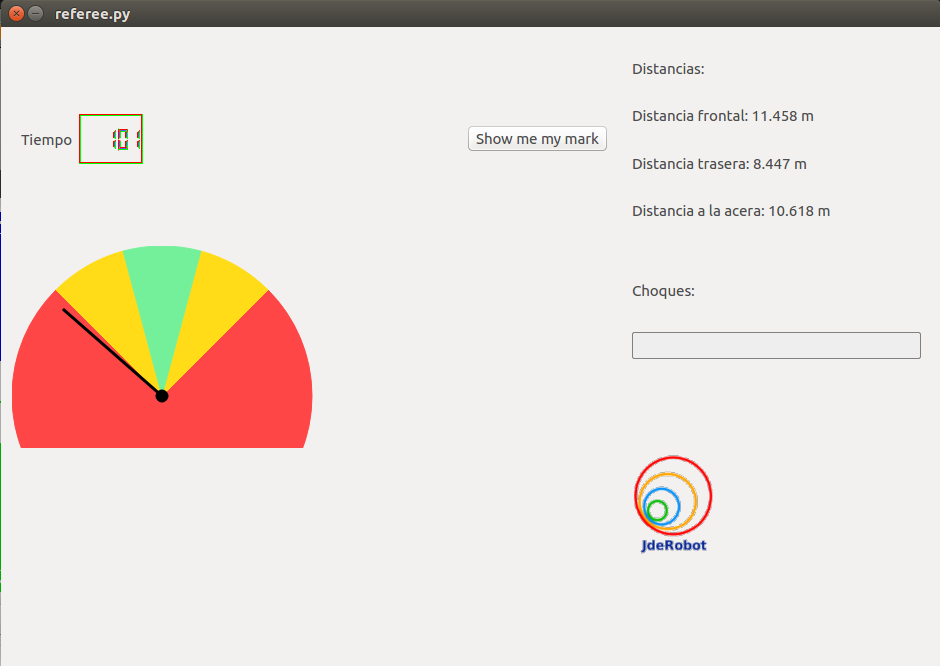
\includegraphics[width=0.6\textwidth]{figures/Autopark/Referee_DurantePractica.png}
		\caption{Evaluador Automático del Autopark durante la ejecución de la práctica}
		\label{fig.Referee_DurantePractica}
		\end{center}
\end{figure}


\section{Experimentación}
La práctica “Aparcamiento automático” se puede ejecutar abriendo tres terminales y escribiendo lo siguiente en cada uno de ellos:

\begin{itemize}
\item Lanzar Gazebo: gazebo autopark.world
\item	Ejecutar la práctica y lanzar la interfaz gráfica (\acrshort{gui}): python2 autopark.py -- --Ice.Config=autopark.cfg
\item	Ejecutar el evaluador automático: python2 referee.py -- --Ice.Config=autopark.cfg
\end{itemize}

Si el ordenador que se emplea no posee muchos recursos se puede arrancar el simulador sin interfaz gráfico:

\begin{itemize}
\item Lanzar Gazebo: gzserver autopark.world
\end{itemize}

En la práctica se han realizado dos pruebas para ver cómo realizaba el taxi el recorrido. Estas pruebas las explicaremos a continuación.\\

En la primera prueba hemos puesto el taxi más alejado de la plaza de aparcamiento para ver si era capaz de conducir hasta encontrar una plaza de aparcamiento y aparcar. El taxi lo hemos desplazado 8 metros más atrás en Gazebo. En las pruebas hemos podido observar que el vehículo era capaz de hacer más recorrido conduciendo hacia delante hasta que encontraba la plaza de aparcamiento y estacionaba de forma correcta. A continuación, podemos ver una secuencia de imágenes del taxi, donde podemos apreciar desde qué posición iniciaba el pilotaje y cómo era capaz de aparcar.

\begin{figure}[H]
  \begin{center}
    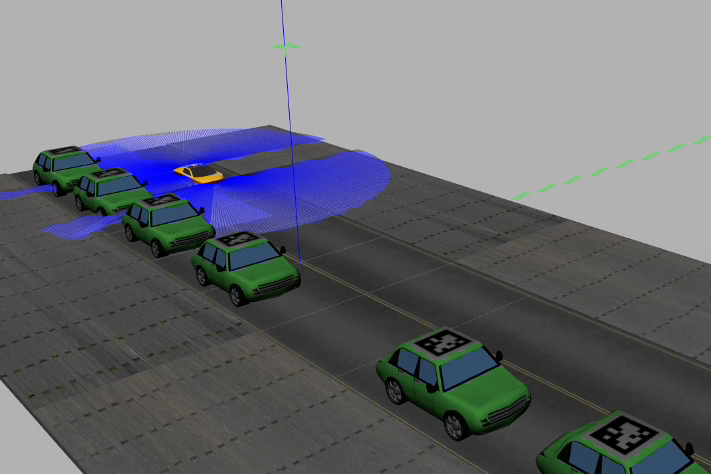
\includegraphics[width=0.7\textwidth]{figures/Autopark/Experimento1_1.png}
		\caption{Taxi en la posición inicial}
		\label{fig.Experimento1_1}
		\end{center}
\end{figure}

\begin{figure}[H]
  \begin{center}
    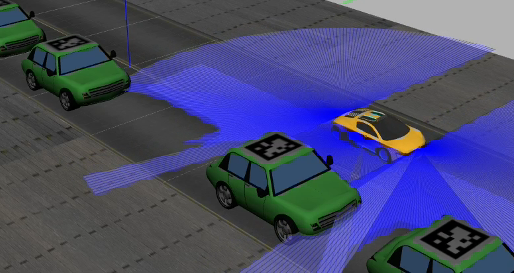
\includegraphics[width=0.7\textwidth]{figures/Autopark/Experimento1_2.png}
		\caption{Taxi parado en paralelo al coche de delante de la plaza de aparcamiento}
		\label{fig.Experimento1_2}
		\end{center}
\end{figure}

\begin{figure}[H]
  \begin{center}
    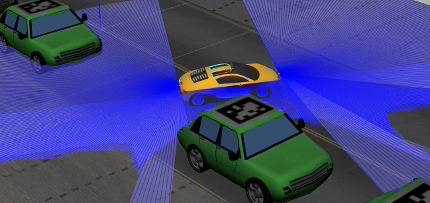
\includegraphics[width=0.7\textwidth]{figures/Autopark/Experimento1_3.png}
		\caption{Taxi realizando maniobras}
		\label{fig.Experimento1_3}
		\end{center}
\end{figure}

\begin{figure}[H]
  \begin{center}
    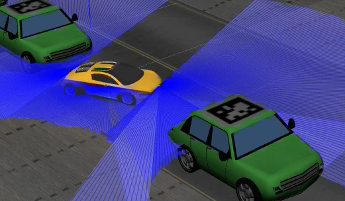
\includegraphics[width=0.7\textwidth]{figures/Autopark/Experimento1_4.png}
		\caption{Taxi realizando maniobras}
		\label{fig.Experimento1_4}
		\end{center}
\end{figure}

\begin{figure}[H]
  \begin{center}
    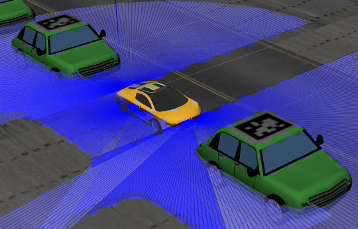
\includegraphics[width=0.6\textwidth]{figures/Autopark/Experimento1_5.png}
		\caption{Taxi aparcado}
		\label{fig.Experimento1_5}
		\end{center}
\end{figure}

En la siguiente prueba se ha desplazado el vehículo hasta tenerlo en paralelo al coche que está delante de la plaza de aparcamiento. En esta prueba se ha comprobado que el coche no avanza hacia delante para buscar una plaza libre de aparcamiento al comienzo como sucedía en la práctica, sino que detecta que hay una plaza libre justo detrás de él y comienza a realizar la maniobra de aparcamiento. Este era el objetivo que se buscaba en esta prueba y el taxi lo ha conseguido con éxito. A continuación, tenemos una secuencia de imágenes que muestran el coche al inicio de la práctica y las maniobras realizadas por el mismo para poder aparcar.

\begin{figure}[H]
  \begin{center}
    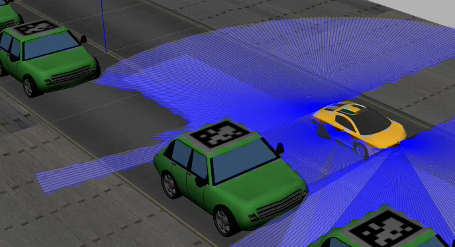
\includegraphics[width=0.6\textwidth]{figures/Autopark/Experimento2_1.png}
		\caption{Posición inicial del taxi al ejecutar la práctica}
		\label{fig.Experimento2_1}
		\end{center}
\end{figure}

\begin{figure}[H]
  \begin{center}
    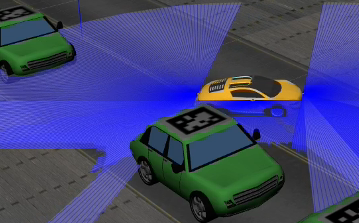
\includegraphics[width=0.6\textwidth]{figures/Autopark/Experimento2_2.png}
		\caption{Taxi realizando maniobras}
		\label{fig.Experimento2_2}
		\end{center}
\end{figure}

\begin{figure}[H]
  \begin{center}
    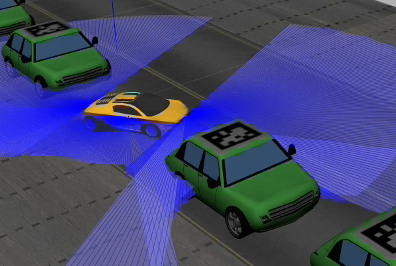
\includegraphics[width=0.6\textwidth]{figures/Autopark/Experimento2_3.png}
		\caption{Taxi realizando maniobras}
		\label{fig.Experimento2_3}
		\end{center}
\end{figure}

\begin{figure}[H]
  \begin{center}
    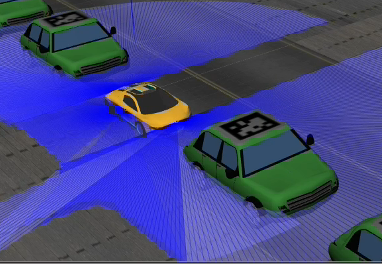
\includegraphics[width=0.6\textwidth]{figures/Autopark/Experimento2_4.png}
		\caption{Taxi estacionado}
		\label{fig.Experimento2_4}
		\end{center}
\end{figure}